%!Tex Root = ../Tutorat3.tex
% ./Packete.tex
% ./Design.tex
% ./Deklarationen.tex
% ./Aufgabe1.tex
% ./Aufgabe2.tex
% ./Aufgabe3.tex
% ./Aufgabe5.tex
% ./Bonus.tex

\section{Task 4}

\setcounter{task}{1}

\if\pascal0{
  \begin{frame}[allowframebreaks]{Task 4}{EDF* - Example}
    \begin{tasknoinc}
  Given tasks $A, B, C, D, E, F, G$ with precedences $A \rightarrow C$, $B \rightarrow C$, $C \rightarrow E$, $D \rightarrow F$, $B \rightarrow D$, $C \rightarrow F$, $D \rightarrow G$.

  All tasks arrive at time $t_0 = 0$, have a common deadline $d = 20$ and the following execution times:
  \begin{center}
  \begin{tabular}{|c|c|c|c|c|c|c|c|c|}
       \hline
       & A & B & C & D & E & F & G\\
       \hline
       \hline
       $C_i$ & 3 & 2 & 4 & 3 & 2 & 5 & 1\\
       \hline
  \end{tabular}
  \end{center}
  We will now prepare the tasks for EDF*
  \end{tasknoinc}
  \end{frame}
}\fi

\begin{frame}{Task 4}{EDF*}
  \if\pascal1{
  \begin{itemize}
      \item EDF* is an alternative version of the EDF Algorithmus
      \item EDF* helps us to schedule Tasks with arbitrary arrival times \alert{\underline{and precedences}}. (contrary to EDF)
      \item EDF* manages this in polynomial time!
  \end{itemize}
  }\else{
  \begin{requirements}
    \begin{itemize}
      \item \alert{preemptive}
      \item \alert{arbitrary arrival times}
      \item tasks are \alert{dependent}
      \item \alert{release time} and \alert{deadline} of individual tasks are modified such that all the \alert{precedence constraints} are satisfied
      \item scheduling problem is \alert{transformed} into a problem \alert{without precedence constraints}, which can then be handled by a "normal" EDF scheduler
    \end{itemize}
  \end{requirements}
  }\fi
\end{frame}

\begin{frame}[allowframebreaks]{Task 4}{EDF* - Transformation}
\begin{itemize}
    \item EDF* transforms the arrival time and deadline of every task in the following way:
    \item[] \alert{Deadline}: \begin{enumerate}
        \item Task must finish the execution time within its deadline: $f_i \leq d_i$
        \item Task must not finish the execution time later than the maximum start time of its successor(s): $f_i \leq d_j - C_j$
        \item[$\rightarrow$] $d_i^* = min(d_i, min(d_j^* - C_j : J_i \rightarrow J_j))$
    \end{enumerate}
    \framebreak
    \item[] \alert{Arrival time} \begin{enumerate}
        \item Task must start the execution not earlier than its release time: $s_j \geq r_j$
        \item Task must not start execution earlier than the minimum finishing time of its predecessor(s): $s_j \geq r_i + C_i$
        \item[$\rightarrow$] $r_j^* = max(r_j, max(r_i^* + C_i : J_i \rightarrow J_j))$
    \end{enumerate}
\end{itemize}
\end{frame}

\if\pascal1{
\begin{frame}[allowframebreaks]{Task 4}{EDF* - Example}
Given tasks $A, B, C, D, E, F, G$ with precedences $A \rightarrow C$, $B \rightarrow C$, $C \rightarrow E$, $D \rightarrow F$, $B \rightarrow D$, $C \rightarrow F$, $D \rightarrow G$.

All tasks arrive at time $t_0 = 0$, have a common deadline $d = 20$ and the following execution times:
\begin{center}
\begin{tabular}{|c|c|c|c|c|c|c|c|c|}
     \hline
     & A & B & C & D & E & F & G\\
     \hline
     \hline
     $C_i$ & 3 & 2 & 4 & 3 & 2 & 5 & 1\\
     \hline
\end{tabular}
\end{center}
We will now prepare the tasks for EDF*
\end{frame}
}\fi

\begin{frame}{Task 4}{EDF* - Precedence graph example}
Given the precedences $A \rightarrow C$, $B \rightarrow C$, $C \rightarrow E$, $D \rightarrow F$, $B \rightarrow D$, $C \rightarrow F$, $D \rightarrow G$ we first draw the precedence graph:
\end{frame}

\begin{frame}{Task 4}{EDF* - Precedence graph example}
\begin{figure}
    \centering
    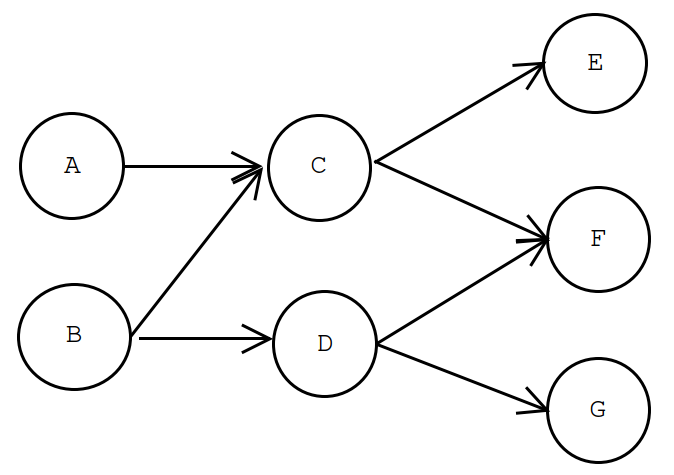
\includegraphics[scale=0.4]{figures/precedencegraph}
    \caption{Task 4: precedence graph}
    \label{pregraph}
\end{figure}
\end{frame}

\begin{frame}[allowframebreaks]{Task 4}{EDF* - Transformation example}
    \begin{itemize}
        \item $r_A^* = r_A$, $r_B^* = r_B$
        \item $r_C^* = \max\{r_C,\max\{r_A^* + C_A, r_B^* + C_B\}\} = \max\{0, \max\{3, 2\}\} = 3$
        \item $r_D^* = \max\{r_D,r_B^* + C_B\} = \max\{0, 2\} = 2$
        \item $r_F^* = \max\{r_F,\max\{r_C^* + C_C, r_D^* + C_D\}\} = \max\{0, \max\{7, 5\}\} = 7$
        \item $r_E^* = \max\{r_E,r_C^* + C_C\} = \max\{0, 7\} = 7$
        \item $r_G^* = \max\{r_G,r_D^* + C_D\} = \max\{0, 5\} = 5$
    \end{itemize}
    \framebreak
    \begin{itemize}
        \item $d_E^* = d_F^* = d_G^* = 20$
        \item $d_C^* = \min\{d_C, \min\{d_E^* - C_E, d_F^* - C_F\}\} = \min\{20, \min\{18, 15\}\} = 15$
        \item $d_D^* = 15$
        \item $d_A^* = 11$
        \item $d_B^* = 11$
    \end{itemize}
    We now successfully have transformed the problem into one without precedence and can simply use EDF!
\end{frame}

\begin{frame}{Task 4}{EDF* - Transformation example}
  \begin{itemize}
    \item The modified \alert{release times} and \alert{deadlines} are:
  \end{itemize}
  \centering
 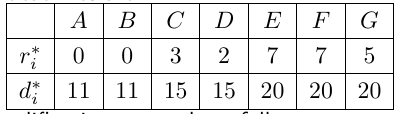
\includegraphics[height=0.2\paperheight]{./figures/4_tab.png}
\end{frame}

\begin{frame}[allowframebreaks]{Task 4}{EDF* - Schedule}
  \begin{tasknoinc}
    \begin{itemize}
      \item determine a resulting EDF* schedule
      \item for this schedule, compute the \alert{average of all response times} of the tasks
    \end{itemize}
  \end{tasknoinc}
  \begin{requirementsnoinc}
    \begin{itemize}
      \item \alert{average response time:} $\displaystyle \overline{t_r}=\frac{1}{n} \sum_{i=1}^n\left(f_i-r_i\right)$
      \begin{itemize}
        \item metric to \alert{compare schedules}
      \end{itemize}
    \end{itemize}
  \end{requirementsnoinc}
\end{frame}

\begin{frame}{Task 4}{EDF* - Schedule}
    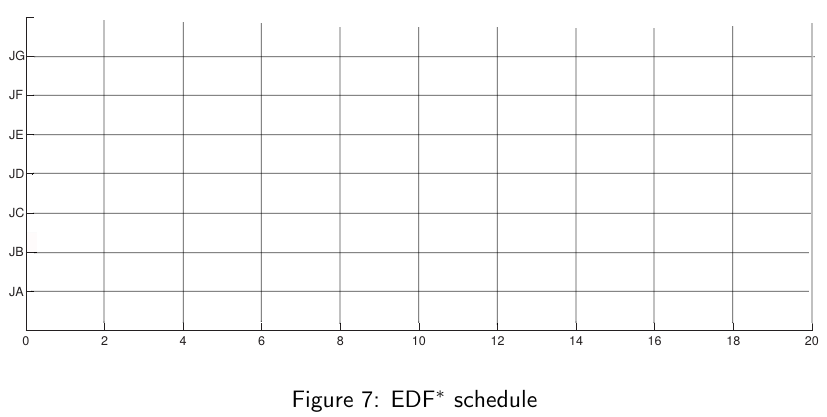
\includegraphics[width = 0.9\linewidth]{figures/EDF-star-schedule.png}
\end{frame}

\begin{frame}{Task 4}{EDF* - Schedule}
    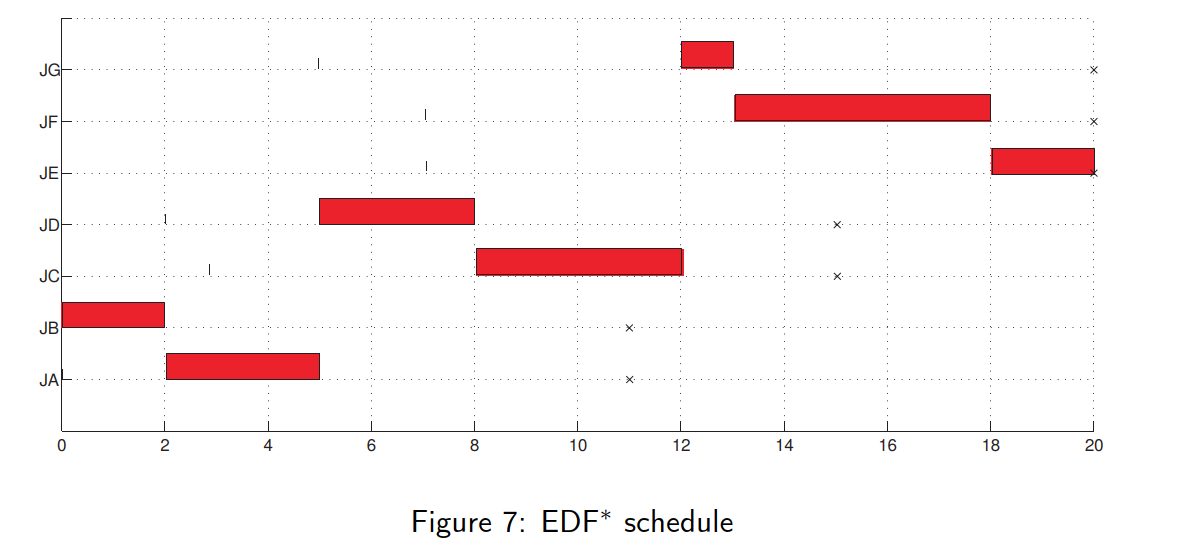
\includegraphics[width = \linewidth]{figures/edf-star-schedule-2.PNG}
\end{frame}

\begin{frame}[allowframebreaks]{Task 4}{EDF* - Schedule}
  \begin{solution}
  \begin{itemize}
    \item $\displaystyle \overline{t_r}=\frac{1}{7} \sum_{i=1}^7\left(f_i-r_i\right)=\frac{5+2+9+6+13+11+8}{7}=\frac{54}{7}=7.714$
    %"a_" + str(5 - 0) ❯ 'a_5'
    % 2 "b_" + str(2 - 0) ❯ 'b_2'
    % 3 "c_" + str(12 - 3) ❯ 'c_9'
    % 4 "d_" + str(8 - 2) ❯ 'd_6'
    % 5 "e_" + str(20 - 7) ❯ 'e_13'
    % 6 "f_" + str(18 - 7) ❯ 'f_11'
    % 7 "g_" + str(13 - 5) ❯ 'g_8'
  \end{itemize}
  \end{solution}
\end{frame}

\begin{frame}[allowframebreaks]{Task 4}{EDF* - Schedule}
  \begin{tasknoinc}
    \begin{itemize}
      \item additional precedence constraint $E \rightarrow A$
      \item still a \alert{feasible schedule} for the task set
    \end{itemize}
  \end{tasknoinc}
  \begin{requirementsnoinc}
    \begin{itemize}
      \item \aalert{Precedence relations} between tasks can be described through an \alert{acyclic} \aalert{directed graph $G$} where tasks are represented by nodes and precedence relations by arrows. G induces a partial order on the task set.
    \end{itemize}
  \end{requirementsnoinc}
  \begin{solutionnoinc}
    \begin{itemize}
      \item No, the task set is no longer schedulable. Under the new conditions, the constraints among tasks A, C
and E introduce a cycle in the precedence graph.
      \item As a result, none of the three tasks can be executed as first and therefore, no feasible schedule exists.
    \end{itemize}
  \end{solutionnoinc}
\end{frame}
